
\begin{figure}
\centerline{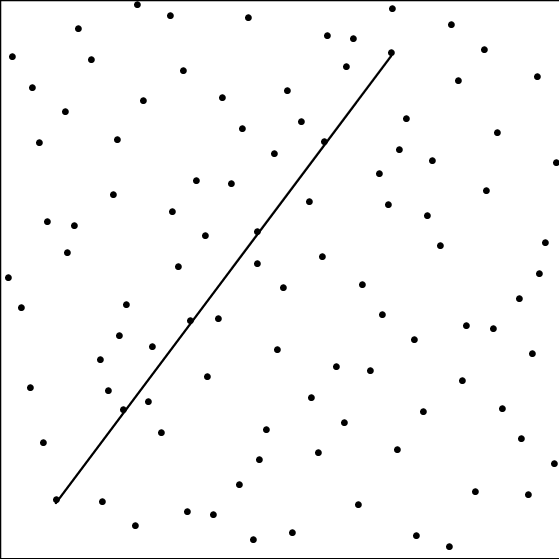
\includegraphics[width=6cm]{../png/hbequisp.png}}
\caption{Conceptual configuration.
A particle, indicated by the straight line, moves against a background thermal (`fluid')
species shown as dots.  In the refinement by De~Esch, interactions take place
at uniformly spaced intervals along the track, also indicated by dots\label{fig:hbequisp}}
\end{figure}

As illustrated in \Fig{hbequisp}, let $\tau (s)$ be the optical depth traversed by a 
article traveling a distance~$s$ through a medium 
with arbitrarily specified macroscopic cross-section~$\sigma(s)$: 
\begin{equation}\label{eq:optd}
\tau(s)= {\int_0}^s \sigma(s')ds'
\end{equation}
We assume only that $\sigma$ is finite and $\sigma(s)\ge 0$. Note that 
\begin{equation}\label{eq:doptd}
\frac{d \tau}{d s} = \sigma (s) 
\end{equation}
To explicitly allow for the case of no collision in a finite distance of travel, 
we define~$\mathrm{P}_{NC}$, the probability of no collisions, as 
\begin{equation}\label{eq:PNC}
\mathrm{P}_{NC} = \exp{(-\tau(\infty))}
\end{equation}
Then the probability density function (pdf) for a collision occurring after a particle has traveled a 
distance~$s$ through the medium is given by~\cite[\S\,7]{lewismiller}
\begin{equation}\label{eq:pdf}
\mathrm{p}(s)=\mathrm{P}_{NC} \delta(s-s_{\infty}) + \frac{d \tau}{d s} \exp{(-\tau(s))}
\end{equation}
where $\frac{d \tau}{d s}$ is the interaction probability per unit distance travelled,
$s_{\infty}$ is the distance to the boundary of the computational domain and
$\exp{(-\tau(s))}$ is the probability of traversing 
distance~$s$ without collision. \Eq{pdf} explicitly allows for cases where 
$\tau(\infty)$ is 
finite, hence there is a possibility of traveling an infinite distance without colliding.

Unbiased random sampling of the Monte Carlo path requires solving the
following for~$s$, distance along the path, 
namely
\begin{equation}\label{eq:xisamp}
\xi = {\int_0}^s \mathrm{p}(s')ds'
\end{equation}
where $\xi$ is sampled from a uniform random variable on~$[0,1)$. In the
spirit of
De~Esch, values of $\xi= j/N_{\xi}, j=1, \ldots N_{\xi}-1$ should be used,
and the charged particle weights (effectively the number of physical
particles each represents) be reduced by~$N_{\xi}$. Values of $N_{\xi} \approx
10-100$ are suggested.
 
In the first step of the sampling, discrete sampling is used to select a collision with probability $(1-\mathrm{P}_{NC})$
or an infinite flight with probability $\mathrm{P}_{NC}$. That is, 
if $\xi > \mathrm{P}_{NC}$, 
then there is a collision. The second step is to sample~$s$ from 
 from the pdf given by:
\begin{equation}\label{eq:partpdf}
g(s')=\frac{1}{G} \frac{d \tau}{d s'}\exp{(-\tau(s'))}
\end{equation}
where
\begin{equation}\label{eq:GPNC}
G= (1-\mathrm{P}_{NC})
\end{equation}
Using \Eq{partpdf}, note that 
\begin{equation}\label{eq:gconstr}
{\int_0}^s g(s')ds' = \frac{1}{G} {\int_0}^{\tau(s)} \exp{(-\tau)}d\tau
\end{equation}
Using \Eqs{xisamp}{partpdf}, we can sample $\tau_s=\tau(s)$ by solving 
\begin{equation}\label{eq:xiG}
\xi=\frac{1}{G} {\int_0}^{\tau_s} \exp{-\tau}d\tau
\end{equation}
This is equivalent to sampling from a truncated exponential pdf, which has 
the solution 
\begin{equation}\label{eq:xiGsoln}
\tau_s -\ln(1-G\xi)
\end{equation}
Pathlength $s$ then follows from \Eq{optd}, viz.
\begin{equation} \label{eq:sfromtau}
\tau_s ={\int_0}^s \sigma(s') ds'
\end{equation}
When $\sigma(s')$ has a simple functional form, \Eq{sfromtau} can often be solved analytically for~$s$. In many 
cases which arise in practice, the solution may involve a transcendental equation or other form 
not amenable to analytic solution. \Eq{sfromtau}, however, can be readily solved numerically for~$s$ 
using Newton iteration with $f= {\int_0}^s \sigma(s') ds' -s$,
starting with an initial estimate $s_0 = \tau_s/\sigma(0)$~\cite{Br03Dire}. 
Because $df/ds\le 0$, $f$ is monotone and there can be at most one root.
For cases where $\sigma(s')\ge 0$,
the Newton iteration is guaranteed to 
converge. However, if $\sigma(s')$ is zero or very small over a portion of the path, $df/ds$~may be~$0$,
leading to numerical difficulties and nonconvergence. This potential problem is 
remedied easily by combining Newton with a bisection search method, such that
bisection is used if $df/ds$ is very small or zero. Using this approach, Brown
and Martin 
found that only $1-5$~iterations are typically needed to converge~$s$ to within
part in $10^6$.
even for extreme variations in $\sigma(s')$. 

 
A final practical point concerns the relation of path length~$s$ to physical coordinates.
If the particle starts at~${\bf x}_0$ and travels in a direction
given by ${\bf v}_p$ parallel to unit vector~${\bf d}$ then the particle path is given by
\begin{equation}\label{eq:patheq}
{\bf x} = {\bf x}_0 + s {\bf d}
\end{equation}
so inverting
\begin{equation}\label{eq:zpatheq}
s = |{\bf x}-{\bf x}_0|/|{\bf d}|
\end{equation}
so it is helpful if ${\bf d}$ is a unit vector.
